\documentclass{cake-classes/short-report-fa}
\usepackage{booktabs}
\begin{document}
\درج‌عنوان‌سند

\قسمت{مقدمه}
در این متن، معماری پیشنهادی برای نسخهٔ اول پلتفرم ابری پروژه کیک روباتیک معرفی شده است.

\قسمت{معماری}

معماری انتخاب شده در شکل \رجوع{معماری} آمده است. بلوک‌های این شکل هر کدام یک سرویس هستند که از یک یا چند میکروسرویس تشکیل می‌شوند. خط سفید به معنای ارتباط دوطرفه و پیکان به معنای جریان داده یک‌طرفه می‌باشد. سرویس‌های زرد رنگ در داخل تیم توسعه داده نمی‌شوند.
همچنین، لازم به ذکر است که در این شکل تنها اتصالات کلیدی ذکر شده است؛ برای مثال، سرویس احراز هویت و دسترسی (\مل{Auth})، تقریبا با تمام سرویس‌های بک‌اند ارتباط دارد که در شکل نیامده است.
در سمت راست نمودار هم سرویس‌های رباتیک ابری دیده می‌شود که هنوز تصمیم‌گیری برای آن‌ها کامل نشده است.

\begin{figure}[t]
	\centering
	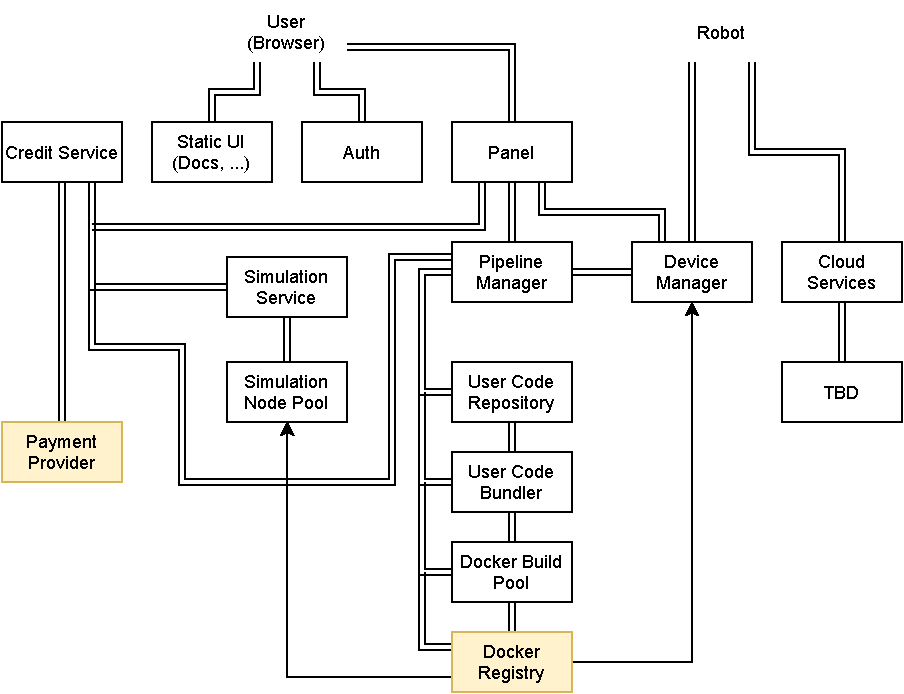
\includegraphics[width=\linewidth]{arch.pdf}
	\شرح{معماری انتخاب شده}
	\برچسب{معماری}
\end{figure}

برای شرح شکل \رجوع{معماری}، از کاربر (\مل{User}) شروع می‌کنیم. کاربر از طریق مرورگر با پلتفرم ارتباط برقرار می‌کند\پانوشت{در حقیقت کاربر می‌تواند با روش‌های جایگزین مانند خط فرمان (\مل{Command Line}) نیز با پلتفرم ارتباط برقرار کند اما در این سند به این موارد نخواهیم پرداخت زیرا تمرکز روی معماری اصلی سیستم و فرایندهای غالب است.} و پیش از لاگین، تنها به صفحه‌ اصلی سایت، مستندات و صفحات ایستای فرعی مانند اطلاعات تماس یا شرایط خدمات دسترسی خواهد داشت. این صفحات در معماری با نام \مل{Static UI} نمایش داده شده‌اند.

برای استفاده از پلتفرم، کاربر با استفاده از سرویس احراز هویت (\مل{Auth}) وارد سیستم می‌شود. این سرویس نام کاربری و رمز عبور را دریافت می‌کند و در صورت صحت آن، یک توکن مدت‌دار ایجاد می‌کند که در حافظهٔ محلی مرورگر کاربر ذخیره می‌شود. این توکن برای احراز هویت کاربر به کار می‌رود. در واقع، کاربر برای استفاده از هر یک از امکانات پلتفرم لازم است این توکن را به همراه درخواست مربوطه ارسال کند. تمام سرویس‌های دیگر نیز باید قبل از دادن خدمات به کاربر، ابتدا از وجود توکن مطمئن شوند. همچنین، این سرویس‌ها باید در صورت وجود توکن ابتدا آن را با ارسال به سرویس \مل{Auth} اعتبارسنجی کنند و مطمئن شوند آن توکن منقضی نشده است و مربوط به کاربر درخواست دهنده است.

سرویس بعدی، سرویس \مل{Panel} است. این سرویس، رابط کاربری اصلی پلتفرم است که کاربر در آن می‌تواند نظارت و مدیریت ربات‌ها، پروژه‌ها و کدها را انجام دهد. این سرویس به چندین سرویس بک‌اند متصل است.

سرویس \مل{Device Manager}، مدیریت ربات‌ها را بر عهده دارد. این سرویس به ربات متصل است. در واقع، ربات هنگام روشن شدن از طریق یک پروتکل اتصال دائمی مانند \مل{WebSocket} این اتصال را ایجاد می‌کند و وضعیت خود را اعلام می‌کند. مواردی نظیر وضعیت ربات، نسخهٔ کد درحال اجرا، و لاگ کد از جمله اطلاعاتی هستند که از ربات به \مل{Device Manager} می‌روند. سرویس \مل{Device Manager} نیز به طور متقابل، دستوراتی نظیر آغاز اجرای کد، توقف اجرای کد و یا به روزرسانی کد از مواردی هستند که از \مل{Device Manager} به ربات می‌روند.

سرویس \مل{Pipeline Manager} که به پنل متصل است، فرایند استقرار کد جدید را مدیریت می‌کند. منظور از پایپ‌لاین، مسیری خودکار است که آغاز آن لحظه‌ای است که کاربر در محیط وب کد را می‌نویسد یا تغییر می‌دهد و روی دکمهٔ \مل{Push to Robot} کلیک می‌کند. پایان این پایپ‌لاین نیز لحظه‌ای است که این کد در ربات اجرا می‌شود.

برای تحقق مدیریت پایپ‌لاین، سرویس \مل{Pipeline Manager} به چند سرویس زیردست متصل است. اولین سرویس، \مل{User Code Repository} است. نقش این سرویس نگهداری کد کاربر و نسخه‌زنی آن است. هر کدی که به ربات می‌رود ابتدا باید در این مکان ذخیره شود.

سپس، سرویس \مل{User Code Bundler} فراخوانی می‌شود. این سرویس، یک \مل{Dockerfile} ایجاد می‌کند که وظیفه ساخت یک ایمیج شامل پلتفرم پایهٔ \مل{ROS}، پکیج‌های \مل{ROS}، پکیج‌های پایتون و کتابخانه کیک را دارد. در واقع این سرویس باید به درستی وابستگی‌های کد را شناسایی کرده و نحوهٔ ارضای آن‌ها را به صورت یک \مل{Dockerfile} در بیاورد. دقت کنید که برخلاف سایر نقاط معماری که جزییات پیاده‌سازی ذکر نشده است، در اینجا تاکید بر این است که از \مل{Docker} استفاده می‌شود. دلیل این امر این است که نمی‌خواهیم معماری بیش از حد انتزاعی شود.

سرویس \مل{Docker Build Pool} وظیفه خواندن \مل{Dockerflie} و ساختن ایمیج‌ها را بر عهده دارد. این ایمیج‌ها سپس در \مل{Docker Registry} ذخیره می‌شوند تا بعدا توسط ربات مستقیما دریافت شوند.

همچنین در سمت راست شکل \رجوع{معماری}، سرویس‌های ابری (\مل{Cloud Services}) به چشم می‌خورند. این سرویس‌ها خدماتی هستند که ربات فقط در لحظهٔ اجرای کد از آن‌ها استفاده می‌کند. سرویس‌هایی مانند پردازش تصویر ابری، پردازش صوت ابری و \مل{SLAM} در این محل قرار می‌گیرند.

در انتهای چپ معماری نیز سرویس \مل{Credit} به چشم می‌خورد که وظیفه دارد اعتبار مالی حساب کاربر را نگهداری کند و هنگامی که کاربر از امکانات پولی استفاده می‌کند، اعتبار را به روز کند. این سرویس همچنین به یک درگاه پرداخت خارجی (\مل{Payment Provider}) متصل است.

در نهایت، سرویس‌هایی برای شبیه‌سازی نیز در معماری به چشم می‌خورند که احتمالا بر پایهٔ \مل{Gazebo} خواهند بود.
\end{document}
